\PassOptionsToPackage{table,xcdraw}{xcolor}

\documentclass[sigconf,review,anonymous]{acmart}
\acmConference[ESEC/FSE 2022]{The 30th ACM Joint European Software Engineering Conference and Symposium on the Foundations of Software Engineering}{14 - 18 November, 2022}{Singapore}

%\documentclass[sigconf,review,anonymous]{acmart}
%\acmConference[ESEC/FSE 2021]{The 29th ACM Joint European Software Engineering Conference and Symposium on the Foundations of Software Engineering}{23 - 27 August, 2021}{Athens, Greece}

%\acmConference[ICSE 2022]{The 44th International Conference on Software Engineering}{May 21–29, 2022}{Pittsburgh, PA, USA}

%\documentclass[sigconf,review, anonymous]{acmart}
%\documentclass[sigconf]{acmart}

\usepackage{booktabs}   %% For formal tables:
                        %% http://ctan.org/pkg/booktabs
\usepackage{caption}
\usepackage{subcaption} %% For complex figures with subfigures/subcaptions
                        %% http://ctan.org/pkg/subcaption
\usepackage{array}
\usepackage{amsmath,amsfonts}
\usepackage{algorithm}
\usepackage[noend]{algpseudocode}
%\usepackage{algorithmic}
\usepackage{graphicx}
\usepackage{textcomp}
\usepackage{float}
\usepackage{listings}
\usepackage{xspace}
\usepackage{multirow}
\usepackage{amsthm}
\newtheorem{definition}{Definition}
\usepackage{balance}

\usepackage{fixltx2e}
\usepackage{hyperref}
\usepackage{enumitem}

\usepackage[skins]{tcolorbox}
\usepackage{xcolor,pifont}
\newcommand*\colourcheck[1]{%
	\expandafter\newcommand\csname #1check\endcsname{\textcolor{#1}{\ding{52}}}%
}
\colourcheck{blue}
\colourcheck{green}
\colourcheck{red}

\newtcolorbox{myframe}[2][]{%
  enhanced,colback=white,colframe=black,coltitle=black,
  sharp corners,
  toprule=1.0pt,
  rightrule=0.3pt,
  leftrule=0pt,
  bottomrule=0pt,
  fonttitle=\itshape\scshape\large,
  left=0pt,right=5pt,top=5pt,bottom=3pt,
  attach boxed title to top right={yshift=-0.3\baselineskip-0.4pt,xshift=-5mm},
  boxed title style={tile,size=minimal,left=0.2mm,right=0.5mm,
    colback=white,before upper=\strut},
  title=#2,#1
}

%\newcommand{\code}[1]{{\footnotesize\textsf{#1}}}
\newcommand{\tool}{\textsc{TDConcord}\xspace}
\newcommand{\irsc}{\textsc{IRSC}\xspace}
\newcommand{\tdcleaner}{\textsc{TDCleaner}\xspace}

\newtheorem{Definition}{Definition}
\newtheorem{Claim}{Claim}
\newtheorem{Lemma}{Lemma}
\newtheorem{Theorem}{Theorem}


\newcolumntype{L}[1]{>{\raggedright\arraybackslash}p{#1}}
\newtheorem{observation}{Observation}
\newtheorem{property}{Property}
\newcommand{\code}[1]{{\footnotesize\texttt{#1}}}
\usepackage{amsthm}
 \definecolor{dkgreen}{rgb}{0,0.6,0}
\definecolor{gray}{rgb}{0.5,0.5,0.5}
\definecolor{mauve}{rgb}{0.58,0,0.82}
\lstset{frame=tb,
  language=Java,
  aboveskip=3mm,
  belowskip=3mm,
  showstringspaces=false,
  columns=flexible,
  basicstyle={\small\ttfamily},
  numbers=left,
  numberstyle=\tiny\color{gray},
  keywordstyle=\color{blue},
  commentstyle=\color{dkgreen},
  stringstyle=\color{mauve},
  breaklines=true,
  breakatwhitespace=true,
  tabsize=4
}



\begin{document}

%\title[{\tool}: Deep Fault Localization with Code Coverage Representation Learning]{{\tool}: Deep Fault Localization with Code Coverage Representation Learning}

\title[Removal of Obsolete TODO Comments With Dual-Task Learning]{Removal of Obsolete TODO Comments with Dual-Task Learning}


%%%---- AUTHORS BLOCK ------

\setcopyright{none}

\settopmatter{printacmref=false, printfolios=false}

\renewcommand\footnotetextcopyrightpermission[1]{} % removes footnote with conference information in first column


%(1) present information sorted in a way that a CNN can "see" patterns
%discriminating between faulty and non faulty statements more easily;

%(2) identify the actual crash statement to the network;

%(3) present more information to the deep neural network in the form of
%a summary of data dependences for each statement as well as source
%embedding; and

%(4) the suspiciousness of a statement is seen taking into account
%relationships to other statement, as opposed to a statement by itself”



%\input{sections/abstract}
\begin{abstract}
Abstract goes here ...
\end{abstract}


%\settopmatter{printacmref=true, printccs=true, printfolios=false}

%\begin{CCSXML}
%<ccs2012>
%<concept>
%<concept_id>10011007.10011006.10011073</concept_id>
%<concept_desc>Software and its engineering~Software maintenance tools</concept_desc>
%<concept_significance>500</concept_significance>
%</concept>
%</ccs2012>
%\end{CCSXML}

%\ccsdesc[500]{Software and its engineering~Software maintenance tools}

%\keywords{Deep Learning; Automated Program Repair; Context-based Code Transformation Learning}


\maketitle

\section{Introduction}
\label{intro:sec}

Writing TODO comments in source code is a common activity by
developers to denote their pending programming tasks in a project. For
example, a developer adds a TODO comment as in {\em ``TODO: print an
  error message if file not found''}. This comment could serve as a
reminder for himself/herself or a notification for other team members
on a pending task. TODO comments are very useful in improving
program comprehension, helping developers understanding the design
and implementation in source code~\cite{souza-sigdoc05,ying-msr05}.

In an ideal practice, after the developer or others perform the task
by adding/modifying the code to print the error message, (s)he will
remove that TODO comment.  It is reported that developers may have
(partially) completed the task described in the TODO comment, however,
did not update or remove it due to several reasons such as time
constraints or
carelessness~\cite{tdcleaner-fse21,wen-icpc19,icomment-sosp07}. Such
an out-of-date TODO comment is called {\em obsolete} when its
corresponding task was accomplished, however the comment itself is not
removed. Obsolete TODO comments can confuse developers and due to
their inconsistent information. They could make developers lose
confidence and reliability of the
code~\cite{tdcleaner-fse21,icomment-sosp07}. In many cases, the
unreliable documentation becomes misleading and causes software
defects in the future~\cite{icomment-sosp07,lintan-icse11}. In brief,
obsolete TODO comments could reduce software quality including code
comprehension and reliability, and increase software maintenance
costs.

Because manually detecting and removing the obsolete TODO comments is
time consuming and tedious, it is highly desirable to develop an
automated approach to detect/remove them as early as possible before
they mislead developers and cause any consequences. However, there is
very limited work on detecting obsolete TODO comments.


three encoders, i.e., TODO Comment Encoder, Code Change Encoder, and
Commit Message Encoder, to embed TODO comments, code changes, and
commit messages into contextualized vectors respectively. TDCleaner
then learns correlations and interactions between them by optimizing
the final probability score. When it comes to online prediction, for a
given TODO comment, we pair it with the associated code change and
commit message, and fit them into the trained TDClearner model to
estimate their matching score.

%% TODO: Add line numbers to motivation example snippets, and update section.

\section{Motivation}
\label{intro:sec}

One of the drawbacks in \tdcleaner is that it's designed to learn
the correlations between inputs of different modalities, i.e., source 
code, and natural language. In this section, we illustrate several 
examples that align with the hypotheses described earlier, where
the  code-change resolves the TODO comment, for which, however, 
\tdcleaner still predicts that it is not obsolete, i.e., has not been 
performed by the developer. Figure~\ref{fig:mex_1} illustrates an 
example in which the TODO comment recommends the developers to ensure that 
the item that is to be appended to the {\em''Backpack''} menu is a valid 
game item. This is adopted, and added through the {\em if-statement} 
(on Line \_\_) in the code-change indicating a concordance between 
the code-change  and the TODO comment. However, the commit 
message in this illustration is very vague, indicating some fix to 
the {\em''Backpack''} menu, which is not in accordance with the TODO 
comment. Such  a non-accordance misleads \tdcleaner towards 
classifying the example as non-obsolete. 

\begin{figure}[t]
	\centering
	\begin{subfigure}{.45\textwidth}
		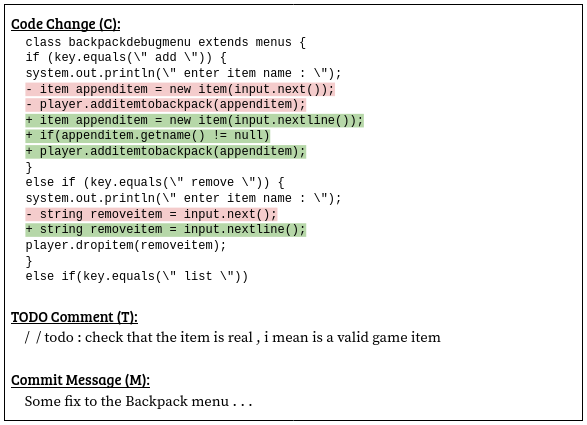
\includegraphics[width=\textwidth]{images/mex_1.png}
		\caption{$T \leftrightarrow C$, $T \nleftrightarrow M$}
		\label{fig:mex_1}
	\end{subfigure}
%%%%%%%%%%%%%%
	\begin{subfigure}{.45\textwidth}
		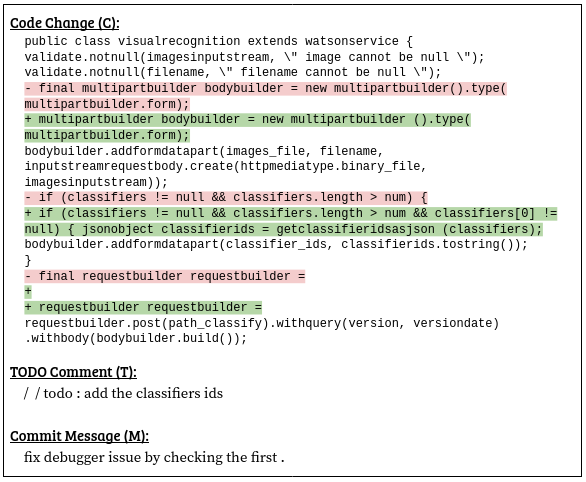
\includegraphics[width=\textwidth]{images/mex_2.png}
		\caption{$T \leftrightarrow C$, $M \geq T$}
		\label{fig:mex_2}
	\end{subfigure}
%%%%%%%%%%%%%%
	\begin{subfigure}{.45\textwidth}
		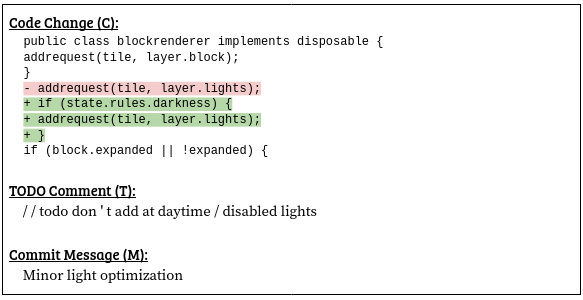
\includegraphics[width=\textwidth]{images/mex_3.png}
		\caption{$T \leftrightarrow C$, $M \geq C$}
		\label{fig:mex_3}
	\end{subfigure}
\caption{Motivating Examples.}
\end{figure}

Figure~\ref{fig:mex_2} illustrates an example in which the TODO comment is
in concordance with the code change, but the commit contains other 
changes as well. The TODO comment recommends the developers 
to add classifier IDs, which is clearly addressed in the statement 
block within the {\em if-statement} on Line \_\_. However, the commit, on 
the whole fixes a debugger issue by adding an additional condition 
to the {\em if-statement}, i.e., by also ensuring that the first element in 
the classifier is not null. This change, overall, also aligns with the 
commit message logged by the developer.

In the example illustrated in Figure~\ref{fig:mex_3}, a developer added a 
TODO comment, to recommend the team to not add requests to a 
block at daytime. This was addressed by introducing a check for 
darkness before adding requests, through the {\em if-statement} on Line
\_\_. However, the corresponding commit message that was logged
for this code modification was very general, indicating a minor
light optimization, which doesn't entirely explain/summarize the 
changes in code. Thus, the contextualized vector learnt for the 
commit message might have acted as noise, influencing \tdcleaner to
predict that the TODO comment in this instance was not addressed
by the developers. 

Such inconsistencies motivated us to explore approaches to 
untangle the $<T, C, M>$ triples, and build individual tasks utilizing 
parts of the triples, each modeled towards detecting obsolete TODO 
comments. This idea forms the crux of \tool, which we'll 
go over in more detail in the following sections.

\section{Our Approach}

\subsection{Problem Statement}

\subsection{Architecture Overview}


\section{Removing Obsolete TODO Comments with \tool}

\subsection{Primary Task \texorpdfstring{(T\textsubscript{p})}{} : \texorpdfstring{<$C$, $T$>}{} Concordance}

%\begin{enumerate}[leftmargin=2em, label=\textbf{\textit{\Alph*.}}]
%    \item \textbf{\textit{CodeBERT for NL-PL pairs.}} 
%    \newline
\subsubsection{CodeBERT for NL-PL pairs.}
The success of transformers-based,
large pre-trained models for natural language processing 
(NLP) tasks prompted researchers to explore the extension 
of such techniques to multi-modal data. In the same spirit, 
Feng et al.~\cite{DBLP:journals/corr/abs-2002-08155} introduced CodeBERT, a bimodal pre-trained 
model for natural language (NL) and programming language 
(PL) pairs. CodeBERT uses the same model architecture as 
RoBERTa-base~\cite{DBLP:journals/corr/abs-1907-11692}, and has a total of 125M parameters.

The segments corresponding to natural language text and 
programming languages are input to CodeBERT, separated 
by special tokens such as {\em [CLS]}, {\em [SEP]}, and {\em [EOS]}. Here, the 
{\em [CLS]} token represents the final hidden representation of the
aggregated sequence representation, {\em [SEP]} token helps 
distinguish between the individual segments, and the {\em [EOS]} token
represents the end of input sequences. Thus, an input to CodeBERT 
looks like {\em [CLS], w\textsubscript{1}, w\textsubscript{2}, ..., w\textsubscript{U} [SEP], c\textsubscript{1}, c\textsubscript{2}, ..., c\textsubscript{V}, [EOS]}, 
where {\em w\textsubscript{i}} correspond to tokens in natural language text, and 
{\em c\textsubscript{j}} correspond to tokens in the programming language. 

%    \vspace{0.8em}
%    \item \textbf{\textit{Code Classification using CodeBERT.}}
%    \newline
\subsubsection{Code Classification using CodeBERT.}
With TODO comments $T$ and the associated code modifications 
$C$ as inputs, we design this task to determine the status 
$S$ of $T$, i.e. predict whether the given $T$ has been addressed by
the developers in $C$ or not:

\begin{equation}
    y = argmax_S P(S|<T, C>)
\end{equation}

Using $T$ and $C$ as the natural language text and programming
language segments respectively, and initializing RoBERTa-base 
model with weights from the pre-trained CodeBERT, we fine-tune 
to the given datasets to encode $<T, C>$ pairs, and effectively 
capture the semantic relationships between them. The final hidden 
state representation of each $<T, C>$ pair is represented by the
corresponding [CLS] token in the model, which we further forward 
to a {\em classification head}. This unit essentially performs a non-linear 
transformation to generate a pooled output for the inputs. The 
output thus generated is used to classify whether a given instance 
is \textit{obsolete} or \textit{non-obsolete}.  Note that we constrain the number of 
tokens in $T$ (i.e., $U$) and $C$ (i.e., $V$) to a maximum length of 128
(i.e., $U \leq 128$ and $V \leq 128$). In addition, the entire input is limited to a 
maximum sequence length of 256 tokens.

%\end{enumerate}

\subsection{Auxiliary Task \texorpdfstring{(T\textsubscript{a})}{} : \texorpdfstring{<$T$, $M$>}{} Concordance}

\subsection{Ensemble Voting Classifier}

\section{Empirical Evaluation}

\subsection{Research Questions}
\par To fully assess \tool's effectiveness in identifying obsolete 
TODO comments, we seek to answer the following research questions:

\begin{enumerate}[leftmargin=3.5em, label=\textbf{RQ\textsubscript{\arabic*} :}]
    \item \textbf{Comparative Analysis.} How does \tool compare
    to other tools proposed for a similar purpose, such as 
    \tdcleaner and \irsc?
    \item \textbf{Why \tool does better?} What are the factors
    that contribute to an improvement in \tool's performance?
    \item \textbf{Ablation Study.} How does removing individual 
    components of the ensemble architecture affect \tool's 
    performance? Can this be extended to better understand it's 
    behavior, and ascertain it's reliability? 
    \item \textbf{Real-World Efficacy of \tool.} How does \tool 
    perform on real-world software projects?
\end{enumerate}

\subsection{Datasets}

\subsection{Methodology}

\subsubsection{RQ\textsubscript{1}: Comparative Analysis}

\subsubsection{RQ\textsubscript{2}: Why \tool does better?}

\subsubsection{RQ\textsubscript{3}: Ablation Study}

\subsubsection{RQ\textsubscript{4}: Real-World Efficacy of \tool}
\section{Experimental Results}
\subsection{\texorpdfstring{RQ\textsubscript{1}}{}: Comparative Analysis}

\subsection{\texorpdfstring{RQ\textsubscript{2}}{}: Why \tool does better?}

\subsection{\texorpdfstring{RQ\textsubscript{3}}{}: Ablation Study}

\subsection{\texorpdfstring{RQ\textsubscript{4}}{}: Real-World Efficacy of \tool}
\section{Related Work}
\section{Conclusion}
\newpage

\balance

%\bibliographystyle{plain}
%\bibliographystyle{ACM-Reference-Format}
\bibliographystyle{ACM-Reference-Format}

\bibliography{References}

\end{document}
